\mode<presentation>
{
  \usetheme{CambridgeUS}
  \usecolortheme{whale}
  \usecolortheme{lily}

  \setbeamercovered{transparent}
  \usefonttheme[onlymath]{serif}
}

\title[\MotorModelingShortName] % (optional, use only with long paper titles)
{\course: \MotorModelingName\license}

\subtitle
{Lecture \MotorModelingNumber} % (optional)


\begin{document}

\begin{frame}
  \titlepage
\end{frame}

\mode<article>{
\maketitle
\tableofcontents
}


%\mode<presentation>{
%\begin{frame}{Outline}
%  \tableofcontents
%  % You might wish to add the option [pausesections]
%\end{frame}}


\section{Pre-requisite Material}
This lecture assumes that the reader is familiar with the following material:
\begin{itemize}
\item Lecture \ModelingMechanicalSystemsNumber:~\ModelingMechanicalSystemsName
\item Lecture \ElectricalSystemsNumber:~\ElectricalSystemsName
\item Lecture \BlockDiagramsNumber:~\BlockDiagramsName
\end{itemize}

%\section{Actuators}
%\begin{frame}{Actuators}
%Some common actuators used in control systems are
%\begin{itemize}
%\item Electric Motors \qquad
%\includegraphics[height=1in]{figures/Motors01CJC}\\<all>
%{\tiny(from http://en.wikipedia.org/wiki/Image:Motors01CJC.jpg. Created by C\_J\_Cowie)}
%\item Hydraulic Actuators \qquad
%\includegraphics[height=1in]{figures/CAT385-Raupenbagger}\\<all>
%{\tiny(http://en.wikipedia.org/wiki/File:CAT385-Raupenbagger.jpg Created by St\"{o}rfix)}
%\end{itemize}
%\end{frame}


\section{Electric Motors}

\begin{frame}{Electric Motors}
\begin{itemize}
\item Motors are {\em transducers} which convert electrical energy to mechanical energy.
\item We will look at models for brushed DC motors.
\end{itemize}
\end{frame}

\subsection{Key Ideas}
\begin{frame}{Key Idea 1: Lorentz Force}
\begin{itemize}
\item An electron moving in a magnetic field experiences a force perpendicular to its motion and the magnetic field.
\begin{center}
$F=q(v\times B)$\hspace{.5in} \begin{minipage}{2in}\includegraphics[height=1.5in]{figures/Cyclotron_motion}\\
{\tiny(http://commons.wikimedia.org/wiki/File:Draaibank.png}
\end{minipage}
\end{center}
\item Electrons move in a circle when exposed to a constant magnetic field.
\end{itemize}
\end{frame}
In the figure, electrons are ejected by the hot-cathode electron gun. Purple light is emitted along the electron path, as gas molecules are excited when collisions with electrons occur. 

\begin{frame}{Key Idea 1: Lorentz Force}
\begin{itemize}
\item Electrons in a wire are constrained to move in a straight line. When a wire is placed in a magnetic field, and a current is set up through the wire, the Lorentz force creates a force perpendicular to the current and the magnetic field.
\begin{center}
$f=Ki$\hspace{.75in} \begin{minipage}{2in}\input{figures/lorentzforce.tex}\end{minipage}
\end{center}
\item This is the basis for a motor - the force on the wire can drive a mechanical load.
\end{itemize}
\end{frame}


\begin{frame}{Key Idea 2: Conservation of Energy}
\begin{columns}
\begin{column}{3in}
\begin{itemize}
\item A force on a wire will cause it to accelerate.
\item Work done
\begin{itemize}
\item on the wire: $\dot{x}f = \dot{x}Ki$.
\item to create the current: $iv_{b}$.
\end{itemize}
\item Conservation of energy suggests these are equal
\begin{align*}
iv_{b} &= \dot{x}Ki,\\
v_{b} &= \dot{x}K.
\end{align*}
\item voltage (back electro-motive force) $v_{b}$  is proportional to the wire's velocity
\end{itemize}
\end{column}
\begin{column}{1.8in}
\begin{center}
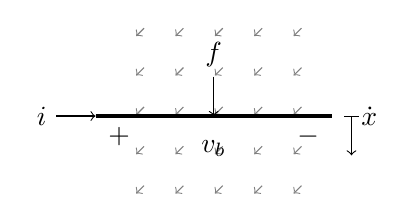
\begin{tikzpicture}[x=1cm,y=1cm,z=-.1cm]
\foreach \x in {0, .5, 1, 1.5, 2}
 \foreach \y in {0, .5, 1, 1.5, 2}
  {
    \draw[->,color=gray] (\x,\y,0) -- (\x,\y,1);
    }
    
 \draw[very thick] (-.5,1,1.15) -- node[pos=.1,below] {$+$} node[pos=.5,below=5pt] {$v_{b}$} node[pos=.9,below] {$-$} (2.5,1,1.15);
 \draw[->] (-1,1,1.15) node[left] {$i$} -- (-.5,1,1.15);
 \draw[->] (1,1.5,1.15) node[above] {$f$} -- (1,1,1.15);
 \draw[|->] (2.75,1,1.15) node[right] {$\dot{x}$} -- ++(0,-0.5,0);
\end{tikzpicture}
\end{center}
\end{column}
\end{columns}
\end{frame}

\begin{frame}{DC motor components}
\begin{center}
\begin{minipage}{1.75in}
\includegraphics[width=1.75in]{figures/DCmotor}\\
{\tiny http://en.wikipedia.org/wiki/File:Motor\_internals.JPG}
\end{minipage}
\begin{minipage}{2.75in}\begin{center}
\begin{tikzpicture}[scale=1.3,inner sep=0pt,outer sep=0pt,very thick]
\draw (0,0) node[fill=black] (a) {}; 
\draw (3.5,0) node[fill=black] (c) {};
\draw (0,-2) node[fill=black] (d) {};
\draw (2,-2) node[fill=black] (e) {};
\draw (3.5,-2) node[fill=black] (f) {};
 
\draw (1,0) node (R1) {\input{\mainfolder/DrawingElements/CircuitElements/resistor.tex}};
\draw (1,0) node[above=.2in] {$R_{a}$};
\draw (2.5,0) node (L1) {\input{\mainfolder/DrawingElements/CircuitElements/inductor.tex}};
\draw (2.5,0) node[above=.2in] {$L_{a}$};
\draw (3.5,-1) node (Rot) {\input{\mainfolder/DrawingElements/CircuitElements/rotor.tex}}; 
\draw[->] (4,-1) ++(0,.5)  node[above=2pt] {$\theta$}  .. controls  ++(-.15,-.3) and ++(-.15,.3) ..  ++(0,-1);
\draw[->] (4.25,-1) ++(0,.5) node[above=2pt] {$\tau_{m}$}  .. controls  ++(-.15,-.3) and ++(-.15,.3) ..  ++(0,-1);


\draw[->] (3.35,-.1) -- node[left=1pt] {$i_{a}$} ++(0,-.5); 
\draw (3.5,-1) node[left=.2in] {$\begin{matrix} + \\ v_{b} \\ -\end{matrix}$};
\draw (0,-1) node (V) {\input{\mainfolder/DrawingElements/CircuitElements/voltagesource.tex}};
\draw (0,-1) node[left=.2in]{$v_{a}$};


%\draw[->] (1.5,-.5) -- node[pos=.5,below=4pt] {$i$} ++(1,0); 

\draw (a) -- (R1);
\draw (R1) -- (L1);
\draw (L1) -| (Rot);
\draw (Rot) -- (f);
\draw (f) -- (d);
\draw (a) -- (V);
\draw (d) -- (V);

\draw (0	,-2.5) node[right] {Motor Constants: $K_{t},K_{e}$};
\draw (0,-3) node[right] {Transducer Relations:};
\draw (3,-3) node[right] {$\boxed{v_{b} = K_{e}\dot{\theta}}$};
\draw (3,-3.5) node[right] {$\boxed{\tau_{m} = K_{t} i_{a} }$};
\end{tikzpicture}

\end{center}
\end{minipage}
\end{center}
\end{frame}

\subsection{Motor Analysis}

\begin{frame}{DC motor diagram}
\begin{center}
\input{figures/motordiagram4.tex}
\end{center}
\end{frame}

This system can be analyzed by finding the equations for the circuit, the equations for the mechanical system, and adding the motor transducer relationships.

\vspace{10pt}
\noindent Circuit:
\[
V_{a}(s) = I_{a}(s)R_{a} + I_{a}(s)L_{a}s + V_{b}(s).
\]
Mechanical System:
\[
Js^{2}\theta(s) = \tau_{m}(s) - bs\theta(s).
\]
Transducer relationships:
\begin{align*}
\tau_{m} &= K_{t}I_{a}(s),\\
V_{b}(s) &= K_{e}s\theta(s).
\end{align*}

A convenient way of viewing these equations is by using a block diagram. 

\subsection{Block Diagram}

The block diagram will relate the variables $V_{a}(s)$, $I_{a}(s)$, $V_{b}(s)$, $\tau_{m}(s)$, and $\theta(s)$. Since $V_{a}(s)$ is an input, we should put it at the left of the block diagram. Note that the circuit equation implies
\[
I_{a}(s) = \frac{1}{R_{a}+L_{a}s}\left(V_{a}(s) - V_{b}(s)\right),
\]
and the mechanical equation implies
\[
\theta(s) = \frac{1}{Js^{2} +bs}\tau_{m}(s).
\]

Using blocks that define the relationships between the variables, we get the following block diagram.
\begin{frame}{DC motor block diagram}
\begin{center}
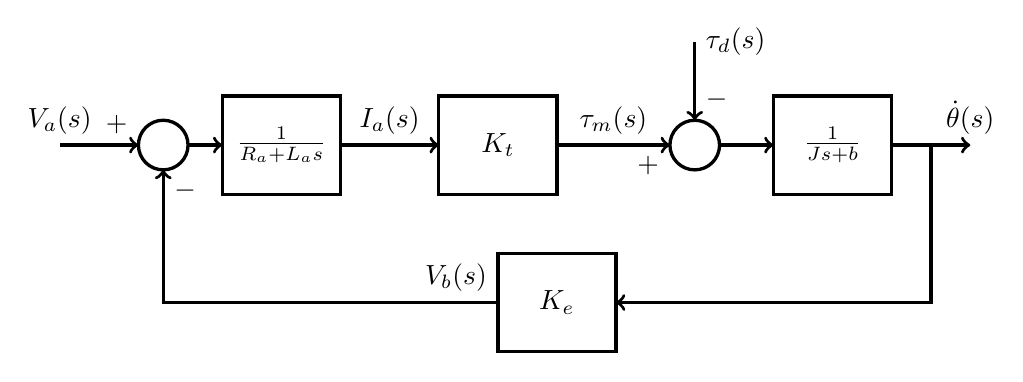
\begin{tikzpicture}[inner sep=0pt,outer sep=0pt,very thick,
sysblock/.style={draw,rectangle,inner sep=2pt,minimum width=1.5cm,minimum height=1.25cm,very thick}]

\draw (0,0) node[draw,circle] (sum) {$\rule{0pt}{18pt}$};
\draw (1.5,0) node[sysblock] (a) {$\frac{1}{R_{a} + L_{a}s}$};
\draw (4.25,0) node[sysblock] (b) {$K_{t}$};
\draw (6.75,0) node[draw,circle] (sum2) {$\rule{0pt}{18pt}$};
\draw (8.5,0) node[sysblock] (c) {$\frac{1}{Js + b}$};
\draw (5,-2) node[sysblock] (d) {$K_{e}$};

\draw[<-] (sum.180) node[above left=4pt] {$+$} -- ++(-1,0) node[above=4pt] {$V_{a}(s)$};
\draw[->] (sum.0) -- (a.180);
\draw[->] (a.0) -- node[pos=.5,above=4pt] {$I_{a}(s)$} (b.180);
\draw[->] (b.0) -- node[pos=.5,above=4pt] {$\tau_{m}(s)$} (sum2.180) node[below left=4pt] {$+$};;
\draw[<-] (sum2.90) node[above right=4pt] {$-$} -- ++(0,1) node[right=4 pt] {$\tau_{d}(s)$};
\draw[->] (sum2.0) -- (c.180);
\draw[->] (c.0) -- ++(1,0) node[above=4pt] {$\dot{\theta}(s)$};
\draw[->] (c.0) -- ++(.5,0) |- (d.0);
\draw[->] (d.180) node[above left=4pt] {$V_{b}(s)$} -| (sum.-90) node[below right=4pt] {$-$};

\end{tikzpicture}
\end{center}
\end{frame}
Note that there is inherent feedback in a DC motor plant system that is \textit{not equivalent to feedback control}. Instead, it is a property of the physical motor system. 

Using this block diagram, you can find the transfer function from $V_{a}(s)$ to any of the other variables.

\subsection{Arbitrary Load}

In the block diagram above, the load was specified to be an inertia with viscous damping. The load came into the block diagram by specifying the mapping from the motor torque $\tau_{m}(s)$ to the rotation of the motor shaft, $\theta(s)$. Note that $\frac{\theta(s)}{\tau_{m}(s)}=N(s)$ defines a mechanical impedance. Thus, we can easily accommodate other loads by substituting in the specific mechanical impedance of the load. 

\begin{frame}{DC motor block diagram with arbitrary load}
\begin{center}
\input{figures/motorblockdiagram2.tex}
\end{center}
\end{frame}

For example, suppose we were given a problem with a different load, say the following:
\begin{frame}{DC motor with different load}
\begin{center}
\input{figures/motordiagram3.tex}
\end{center}
\end{frame}

All we need to do is mentally disconnect the motor, and find the transfer function $\frac{\theta(s)}{\tau_{m}(s)}$. In this case, the load impedance would be found from the network:
\begin{frame}
\begin{center}
\begin{tikzpicture}[inner sep=0pt, outer sep=0pt,very thick]
\draw (0,0) node[draw,fill,inner sep=0pt,outer sep=0pt,circle] (T1) {$\rule{2pt}{0pt}$};
\draw (T1.0) node[above=4pt, inner sep=1pt] {$\theta$};
%\draw (3,0) node[draw,fill,inner sep=0pt,outer sep=0pt,circle] (T2) {$\rule{2pt}{0pt}$};
\draw (3,0) node[draw,fill,inner sep=0pt,outer sep=0pt,circle] (T2) {};
\draw (T2.0) node[above=4pt, inner sep=1pt] {$\theta_{2}$};
\draw (2.75,-2.5) node[draw,fill,inner sep=0pt,outer sep=0pt,circle] (Gnd) {$\rule{2pt}{0pt}$};
\draw (Gnd) node[rotate=90,below,scale=.75] {\input{\mainfolder/DrawingElements/CircuitElements/ground.tex}};


\draw (1.5,0) node (k) {\documentclass[12pt]{article}
% \newcommand{\mainfolder}{/Users/coulston/Dropbox/EENG307Current}  	                    % @ Work PC
%\newcommand{\mainfolder}{C:/Users/Chris/Dropbox/Mycourses/EENG307Current}  	% @ Work Laptop
\newcommand{\mainfolder}{C:/Users/chris/Dropbox/Mycourses/EENG307Current}		% @ Home PC

% \newcommand{\mainfolder}{$HOME/Dropbox/EENG307Current}
\newcommand{\commonmaterial}{\mainfolder/CommonMaterial}
\input{\mainfolder/Headers/packageheader}
\input{\mainfolder/Headers/coursedefheader}

\usepackage{pbox}
%\usepackage{siunitx}
%\usepackage{draftwatermark}
%\SetWatermarkText{DRAFT}
%\SetWatermarkScale{1}

\setlength{\topmargin}{-.75in}
\setlength{\textheight}{9.25in}
\setlength{\oddsidemargin}{-0.25in}
\setlength{\evensidemargin}{-0.25in}
\setlength{\textwidth}{7in}




\begin{document}



%%%%%%%%%%%%%%%%%%%%%%%%%%%%%%%%%%%
\begin{frame}{Electrical Impedance}%
\begin{center}%
\mode<article>{

\begin{tabular}{c|ccc}
 & resistor & capacitor & inductor  \\\hline
 Component & \input{./figures/resistor.tex} & \input{./figures/capacitor.tex} & \input{./figures/inductor.tex}\\\hline
\rule[-8pt]{0pt}{0pt}\rule{0pt}{14pt} 
Component law & $v_1-v_2=iR$ & $i = C\frac{d(v_1-v_2)}{dt}$ & $v_1-v_2=L\frac{di}{dt}$  \\\hline
\rule[-8pt]{0pt}{0pt}\rule{0pt}{14pt} 
Laplace Transform & $V(s)= I(s)R$ & $V(s) = \frac{1}{Cs}I(s)$ & $V(s) = LsI(s)$ \\\hline
Impedance Component & \input{./figures/resistorimpedance.tex} & \input{./figures/capacitorimpedance.tex} & \input{./figures/inductorimpedance.tex}

\end{tabular}}
\end{center}
\end{frame}


%%%%%%%%%%%%%%%%%%%%%%%%%%%%%%%%%%%
\begin{frame}{Fluid Impedance}
\graphicspath{}
\begin{center}
\mode<article>{

\begin{tabular}{c|cc}
 & valve & tank \\\hline
%Component &\begin{tikzpicture}
\draw (.75,0) node (valve) {\input{\mainfolder/DrawingElements/FluidElements/valve.tex}};
\draw (.75,0) node[above=9pt] {$R$};
\draw (-.2,.25) node[above] {$p_{1}$};
\draw[<-] (valve.180) --  ++(-.5,0) node[left] {$q$};
\draw[->] (valve.0) -- ++(.5,0)  node[right] {$q$};
\draw (1.7,.25) node[above] {$p_{2}$};
\draw (.75,1.5) node {$p = p_{1}-p_{2}$};
\end{tikzpicture} &  \input{./figures/figurestank2.tex} \\\hline
Component &\begin{tikzpicture}
\draw (.75,0) node (valve) {\input{\mainfolder/DrawingElements/FluidElements/valve.tex}};
\draw (.75,0) node[above=9pt] {$R$};
\draw (-.2,.25) node[above] {$p_{1}$};
\draw[<-] (valve.180) --  ++(-.5,0) node[left] {$q$};
\draw[->] (valve.0) -- ++(.5,0)  node[right] {$q$};
\draw (1.7,.25) node[above] {$p_{2}$};
\draw (.75,1.5) node {$p = p_{1}-p_{2}$};
\end{tikzpicture} &  \input{./figures/tank.tex} \\\hline
\rule[-8pt]{0pt}{0pt}\rule{0pt}{14pt} Component law & $p=Rq$ & $\frac{A}{\rho g}\frac{dp}{dt} = q_{1} - q_{2}$ \\\hline
\rule[-8pt]{0pt}{0pt}\rule{0pt}{14pt} Laplace Transform & $P(s)= RQ(s)$ & $\frac{A}{\rho g}sP(s) = Q_{1}(s)-Q_{2}(s)$ \\\hline
 Impedance Component & \input{./figures/valveanalogycopy.tex} & \input{./figures/tankanalogycopy.tex}
 \end{tabular}}
 
\mode<presentation>{\resizebox{11cm}{!}{

\begin{tabular}{c|cc}
 & valve & tank \\\hline
Component &\begin{tikzpicture}
\draw (.75,0) node (valve) {\input{\mainfolder/DrawingElements/FluidElements/valve.tex}};
\draw (.75,0) node[above=9pt] {$R$};
\draw (-.2,.25) node[above] {$p_{1}$};
\draw[<-] (valve.180) --  ++(-.5,0) node[left] {$q$};
\draw[->] (valve.0) -- ++(.5,0)  node[right] {$q$};
\draw (1.7,.25) node[above] {$p_{2}$};
\draw (.75,1.5) node {$p = p_{1}-p_{2}$};
\end{tikzpicture} & \input{./figures/tank2.tex} \\\hline
\rule[-8pt]{0pt}{0pt}\rule{0pt}{14pt} Component law & $p=Rq$ & $\frac{A}{\rho g}\frac{dp}{dt} = q_{1} - q_{2}$ \\\hline
\rule[-8pt]{0pt}{0pt}\rule{0pt}{14pt} Laplace Transform & $P(s)= RQ(s)$ & $\frac{A}{\rho g}sP(s) = Q_{1}(s)-Q_{2}(s)$ \\\hline
 Impedance Component & \input{./figures/valveanalogycopy.tex} & \input{./figures/tankanalogycopy.tex}
 \end{tabular}}}
\end{center}
\end{frame}

\pagebreak

%%%%%%%%%%%%%%%%%%%%%%%%%%%%%%%%%%%
\begin{frame}{Mechanical Impedance}%
\begin{center}%
\mode<article>{\begin{tabular}{c|ccc}
 & mass & spring & damper \\\hline
 Component & \begin{tikzpicture}
%  \draw(-1,2.5) node (text) {\textsf{fixed point}};
%   \draw[->] (text.180) -- ++(-.7,0);
   \draw[inner sep=0pt,outer sep=0pt,very thick] (-3,1) node (gnd1) {\input{\mainfolder/DrawingElements/MechanicalElements/ground.tex}};
   \draw[->|,dotted] (-3,1.75) -- node[pos=.5,above] {$x_{f}$} ++(3.6,0); 
    \draw[very thick] (0,0) rectangle (1.2,1);
    \draw (.6,.5) node {$m$};
    \draw[->,thick] (1.2,.5) -- ++(.5,0) node[right] {$f$};
    \draw[|->,thick] (.6,1.2) node[above=2pt] {$x$} -- ++(.5,0);  
\end{tikzpicture}
 & \begin{tikzpicture}
\draw (.75,0) node[inner sep=0,outer sep=0] (K1) {\input{\mainfolder/DrawingElements/MechanicalElements/spring.tex}};
\draw (K1)  node[above=6pt] {$k$};
\draw[very thick] (K1.180) -- ++(-.2,0);
\draw[very thick] (K1.0) -- ++(0.2,0);
\draw[<-,thick] (K1.0) ++(.2,0) -- ++(.5,0) node[right] {$f$};
\draw[<-,thick] (K1.180) ++(-.2,0) -- ++(-.5,0) node[left] {$f$};
\draw[|->,thick] (K1.180) ++(-.2,.4) node[above=2pt] {$x_{1}$} -- ++(.5,0);  
\draw[|->,thick] (K1.0) ++(.2,.4) node[above=2pt] {$x_{2}$} -- ++(.5,0);  
\draw<2-> (K1) ++(0,-.6) node {$f=k(x_{1}-x_{2})$};
\end{tikzpicture}
 & \begin{tikzpicture}
\draw[very thick] (-.2,0) -- (0,0);
\draw (.75,0) node {\input{\mainfolder/DrawingElements/MechanicalElements/damper.tex}};
\draw (.75,0) node[above=9pt] {$b$};
\draw[very thick] (1.5,0) -- ++(.2,0);
    \draw[<-,thick] (1.5,0) ++(.2,0) -- ++(.5,0) node[right] {$f$};
    \draw[<-,thick] (-.2,0) -- ++(-.5,0) node[left] {$f$};
    \draw[|->,thick] (-.2,.4) node[above=2pt] {$x_{1}$} -- ++(.5,0);  
    \draw[|->,thick] (1.7,.4) node[above=2pt] {$x_{2}$} -- ++(.5,0);  
    \draw (.6,-.6) node {$x=x_{1}-x_{2}$};
  %  \draw (.6,-1.2) node {$f=b\dot{x}$};
\end{tikzpicture}\\\hline
\rule[-8pt]{0pt}{0pt}\rule{0pt}{14pt} 
Component law & $f = m\ddot{x}$ & $f = kx$ & $f=b\dot{x}$  \\\hline
\rule[-8pt]{0pt}{0pt}\rule{0pt}{14pt} Laplace Transform & $X(s)= \frac{1}{ms^{2}}F(s)$ & $X(s) = \frac{1}{k}F(s)$ & $X(s) = \frac{1}{bs}F(s)$ \\\hline
\begin{minipage}[b]{1.5in}\begin{center}Impedance Component \\
(positive $f$ direction agrees with positive $x$ direction)\end{center}
\end{minipage}
& \input{figures/massimpedance.tex} & \input{figures/springimpedance.tex} & \input{figures/damperimpedance.tex}
 \end{tabular}}
\mode<presentation>{\resizebox{10cm}{!}{\begin{tabular}{c|ccc}
 & mass & spring & damper \\\hline
 Component & \begin{tikzpicture}
%  \draw(-1,2.5) node (text) {\textsf{fixed point}};
%   \draw[->] (text.180) -- ++(-.7,0);
   \draw[inner sep=0pt,outer sep=0pt,very thick] (-3,1) node (gnd1) {\input{\mainfolder/DrawingElements/MechanicalElements/ground.tex}};
   \draw[->|,dotted] (-3,1.75) -- node[pos=.5,above] {$x_{f}$} ++(3.6,0); 
    \draw[very thick] (0,0) rectangle (1.2,1);
    \draw (.6,.5) node {$m$};
    \draw[->,thick] (1.2,.5) -- ++(.5,0) node[right] {$f$};
    \draw[|->,thick] (.6,1.2) node[above=2pt] {$x$} -- ++(.5,0);  
\end{tikzpicture}
& \begin{tikzpicture}
\draw (.75,0) node[inner sep=0,outer sep=0] (K1) {\input{\mainfolder/DrawingElements/MechanicalElements/spring.tex}};
\draw (K1)  node[above=6pt] {$k$};
\draw[very thick] (K1.180) -- ++(-.2,0);
\draw[very thick] (K1.0) -- ++(0.2,0);
\draw[<-,thick] (K1.0) ++(.2,0) -- ++(.5,0) node[right] {$f$};
\draw[<-,thick] (K1.180) ++(-.2,0) -- ++(-.5,0) node[left] {$f$};
\draw[|->,thick] (K1.180) ++(-.2,.4) node[above=2pt] {$x_{1}$} -- ++(.5,0);  
\draw[|->,thick] (K1.0) ++(.2,.4) node[above=2pt] {$x_{2}$} -- ++(.5,0);  
\draw<2-> (K1) ++(0,-.6) node {$f=k(x_{1}-x_{2})$};
\end{tikzpicture}
 & \begin{tikzpicture}
\draw[very thick] (-.2,0) -- (0,0);
\draw (.75,0) node {\input{\mainfolder/DrawingElements/MechanicalElements/damper.tex}};
\draw (.75,0) node[above=9pt] {$b$};
\draw[very thick] (1.5,0) -- ++(.2,0);
    \draw[<-,thick] (1.5,0) ++(.2,0) -- ++(.5,0) node[right] {$f$};
    \draw[<-,thick] (-.2,0) -- ++(-.5,0) node[left] {$f$};
    \draw[|->,thick] (-.2,.4) node[above=2pt] {$x_{1}$} -- ++(.5,0);  
    \draw[|->,thick] (1.7,.4) node[above=2pt] {$x_{2}$} -- ++(.5,0);  
    \draw (.6,-.6) node {$x=x_{1}-x_{2}$};
  %  \draw (.6,-1.2) node {$f=b\dot{x}$};
\end{tikzpicture}\\\hline
\rule{0pt}{14pt} Component law & $M\ddot{x}=f$ & $f = kx$ & $f=b\dot{x}$  \\\hline
\rule[-8pt]{0pt}{0pt}\rule{0pt}{14pt} Laplace Transform & $X(s)= \frac{1}{Ms^{2}}F(s)$ & $X(s) = \frac{1}{k}F(s)$ & $X(s) = \frac{1}{bs}F(s)$ \\\hline
\begin{minipage}[b]{1.5in}\begin{center}Impedance Component \\
(positive $f$ direction agrees with positive $x$ direction)\end{center}
\end{minipage}
& \input{./figures/massimpedance.tex} & \input{./figures/springimpedance.tex} & \input{./figures/damperimpedance.tex}
 \end{tabular}}}
\end{center}
\end{frame}


%%%%%%%%%%%%%%%%%%%%%%%%%%%%%%%%%%%
\begin{frame}{Rotational Impedance}
\begin{center}
\mode<article>{\begin{tabular}{c|ccc}
 & mass & spring & damper \\\hline
 Component & \begin{minipage}[b]{.75in}\begin{tikzpicture}
    \draw[very thick] (.5,0) node[cylinder,draw,shape aspect=.55,minimum width=1cm,minimum height=1.5cm] (J) {$J$};
    \draw[->] (-.2,.5) node[above] {$\theta$}  .. controls  ++(-.15,-.3) and ++(-.15,.3) ..  ++(0,-1);
    \draw[->] (1.4,-.5) node[below] {$\tau$}  .. controls  ++(.15,.3) and ++(.15,-.3) ..  ++(0,1);
    \draw (.5,-1) node {$J\ddot{\theta}=\tau$};
\end{tikzpicture}\\\vspace{.1in}\end{minipage} & \begin{tikzpicture}
\draw[very thick] (-.2,0) -- (0,0);
\draw (.75,0) node {\input{\mainfolder/DrawingElements/MechanicalElements/spring.tex}};
\draw[very  thick] (1.5,0) -- ++(.2,0);
\draw (.75,0) node[above=9pt] {$k$};
\draw[->] (-.2,.5) node[above] {$\theta_{1}$}  .. controls  ++(-.15,-.3) and ++(-.15,.3) ..  ++(0,-1);
\draw[->] (-.5,.5) node[above] {$\tau$}  .. controls  ++(-.15,-.3) and ++(-.15,.3) ..  ++(0,-1);
\draw[->] (1.5,.5) node[above] {$\theta_{2}$}  .. controls  ++(-.15,-.3) and ++(-.15,.3) ..  ++(0,-1);
\draw[->] (1.9,.5) node[above] {$\tau$}  .. controls  ++(.15,-.3) and ++(.15,.3) ..  ++(0,-1);
\draw (.5,-1) node {$\theta=\theta_{1} - \theta_{2}$};
\end{tikzpicture} & \begin{tikzpicture}
\draw[very thick] (-.2,0) -- (0,0);
\draw (.75,0) node {\input{\mainfolder/DrawingElements/MechanicalElements/damper.tex}};
\draw[very  thick] (1.5,0) -- ++(.2,0);
\draw (.75,0) node[above=9pt] {$b$};
\draw[->] (-.2,.5) node[above] {$\theta_{1}$}  .. controls  ++(-.15,-.3) and ++(-.15,.3) ..  ++(0,-1);
\draw[->] (-.5,.5) node[above] {$\tau$}  .. controls  ++(-.15,-.3) and ++(-.15,.3) ..  ++(0,-1);
\draw[->] (1.5,.5) node[above] {$\theta_{2}$}  .. controls  ++(-.15,-.3) and ++(-.15,.3) ..  ++(0,-1);
\draw[->] (1.9,.5) node[above] {$\tau$}  .. controls  ++(.15,-.3) and ++(.15,.3) ..  ++(0,-1);
\draw (.5,-1) node {$\dot{\theta}=\dot{\theta}_{1} - \dot{\theta}_{2}$};
\end{tikzpicture}\\\hline
 \rule[-8pt]{0pt}{0pt}\rule{0pt}{12pt} 
 Component Law & $\tau = J\ddot{\theta}$ & $\tau = k\theta$ & $\tau = b\dot{\theta}$ \\\hline
\rule[-8pt]{0pt}{0pt}\rule{0pt}{14pt} Laplace Transform & $\theta(s)= \frac{1}{Js^{2}}\tau(s)$ & $\theta(s) = \frac{1}{k}\tau(s)$ & $\theta(s) = \frac{1}{bs}\tau(s)$ \\\hline
\begin{minipage}[b]{1.5in}\begin{center}Impedance Component
\end{center}
\end{minipage}
& \begin{tikzpicture}
\draw (0,0) node (R) {\begin{tikzpicture}
\draw (0,0) node[circle,fill,inner sep=1pt,] {} node[above] {$\theta$};
\draw[very thick] (0,0)  -- ++(0,-.37);
\draw[very thick] (0,-1) node[rectangle,draw,minimum width=.1in,minimum height=.5in] {};
\draw[very thick] (0,-1.65) -- ++(0,-.37);
\draw[very thick] (0,-2) node{\input{\mainfolder/DrawingElements/CircuitElements/elground.tex}};
\end{tikzpicture}
};

\draw (R) node[right=6pt] {$\frac{1}{Js^{2}}$};
%\draw (6.1,.75) node[above] {$+$};
\draw (1,0) node[right] {$\begin{matrix} + \\ \\ \theta(s)\\  \\ - \end{matrix}$};
%\draw (7.9,.75) node[above] {$-$};
\draw[->] (-.3,.5) -- node[pos=.5,left] {$\tau(s)$} ++(0,-1);  

\end{tikzpicture} & \begin{tikzpicture}
\draw (7,.2) node (R) {\begin{tikzpicture}
\draw (0,0) node[circle,fill,inner sep=1pt,] {} node[above] {$\theta_{1}$};
\draw[very thick] (0,0) -- ++(.37,0);
\draw[very thick] (1,0) node[rectangle,draw,minimum width=.5in,minimum height=.1in] {};
\draw[very thick] (1.65,0) -- ++(.37,0);
\draw (2.02,0) node[circle,fill,inner sep=1pt,] {} node[above] {$\theta_{2}$};
\end{tikzpicture}
};
\draw (R) node[above=1pt] {$\frac{1}{k}$};
%\draw (6.1,.75) node[above] {$+$};
%\draw (7,.75) node[above] {$X(s)$};
%\draw (7.9,.75) node[above] {$-$};
\draw[->] (6.5,-.3) -- node[pos=.5,below] {$\tau(s)$} ++(1,0);  
\draw (7,-1.5) node[above] {$\begin{matrix} + & \theta(s) & - \end{matrix}$};

\end{tikzpicture} & \input{./figures/rotdamperimpedance.tex}
 \end{tabular}}
\mode<presentation>{\resizebox{10cm}{!}{\begin{tabular}{c|ccc}
 & mass & spring & damper \\\hline
 Component & \begin{tikzpicture}
    \draw[very thick] (.5,0) node[cylinder,draw,shape aspect=.55,minimum width=1cm,minimum height=1.5cm] (J) {$J$};
    \draw[->] (-.2,.5) node[above] {$\theta$}  .. controls  ++(-.15,-.3) and ++(-.15,.3) ..  ++(0,-1);
    \draw[->] (1.4,-.5) node[below] {$\tau$}  .. controls  ++(.15,.3) and ++(.15,-.3) ..  ++(0,1);
    \draw (.5,-1) node {$J\ddot{\theta}=\tau$};
\end{tikzpicture} & \begin{tikzpicture}
\draw[very thick] (-.2,0) -- (0,0);
\draw (.75,0) node {\input{\mainfolder/DrawingElements/MechanicalElements/spring.tex}};
\draw[very  thick] (1.5,0) -- ++(.2,0);
\draw (.75,0) node[above=9pt] {$k$};
\draw[->] (-.2,.5) node[above] {$\theta_{1}$}  .. controls  ++(-.15,-.3) and ++(-.15,.3) ..  ++(0,-1);
\draw[->] (-.5,.5) node[above] {$\tau$}  .. controls  ++(-.15,-.3) and ++(-.15,.3) ..  ++(0,-1);
\draw[->] (1.5,.5) node[above] {$\theta_{2}$}  .. controls  ++(-.15,-.3) and ++(-.15,.3) ..  ++(0,-1);
\draw[->] (1.9,.5) node[above] {$\tau$}  .. controls  ++(.15,-.3) and ++(.15,.3) ..  ++(0,-1);
\draw (.5,-1) node {$\theta=\theta_{1} - \theta_{2}$};
\end{tikzpicture} & \begin{tikzpicture}
\draw[very thick] (-.2,0) -- (0,0);
\draw (.75,0) node {\input{\mainfolder/DrawingElements/MechanicalElements/damper.tex}};
\draw[very  thick] (1.5,0) -- ++(.2,0);
\draw (.75,0) node[above=9pt] {$b$};
\draw[->] (-.2,.5) node[above] {$\theta_{1}$}  .. controls  ++(-.15,-.3) and ++(-.15,.3) ..  ++(0,-1);
\draw[->] (-.5,.5) node[above] {$\tau$}  .. controls  ++(-.15,-.3) and ++(-.15,.3) ..  ++(0,-1);
\draw[->] (1.5,.5) node[above] {$\theta_{2}$}  .. controls  ++(-.15,-.3) and ++(-.15,.3) ..  ++(0,-1);
\draw[->] (1.9,.5) node[above] {$\tau$}  .. controls  ++(.15,-.3) and ++(.15,.3) ..  ++(0,-1);
\draw (.5,-1) node {$\dot{\theta}=\dot{\theta}_{1} - \dot{\theta}_{2}$};
\end{tikzpicture}\\\hline
\rule[-8pt]{0pt}{0pt}\rule{0pt}{14pt} Laplace Transform & $\theta(s)= \frac{1}{Js^{2}}\tau(s)$ & $\theta(s) = \frac{1}{k}\tau(s)$ & $\theta(s) = \frac{1}{bs}\tau(s)$ \\\hline
\begin{minipage}[b]{1.5in}\begin{center}Impedance Component 
\end{center}
\end{minipage}
& \begin{tikzpicture}
\draw (0,0) node (R) {\begin{tikzpicture}
\draw (0,0) node[circle,fill,inner sep=1pt,] {} node[above] {$\theta$};
\draw[very thick] (0,0)  -- ++(0,-.37);
\draw[very thick] (0,-1) node[rectangle,draw,minimum width=.1in,minimum height=.5in] {};
\draw[very thick] (0,-1.65) -- ++(0,-.37);
\draw[very thick] (0,-2) node{\input{\mainfolder/DrawingElements/CircuitElements/elground.tex}};
\end{tikzpicture}
};

\draw (R) node[right=6pt] {$\frac{1}{Js^{2}}$};
%\draw (6.1,.75) node[above] {$+$};
\draw (1,0) node[right] {$\begin{matrix} + \\ \\ \theta(s)\\  \\ - \end{matrix}$};
%\draw (7.9,.75) node[above] {$-$};
\draw[->] (-.3,.5) -- node[pos=.5,left] {$\tau(s)$} ++(0,-1);  

\end{tikzpicture} & \begin{tikzpicture}
\draw (7,.2) node (R) {\begin{tikzpicture}
\draw (0,0) node[circle,fill,inner sep=1pt,] {} node[above] {$\theta_{1}$};
\draw[very thick] (0,0) -- ++(.37,0);
\draw[very thick] (1,0) node[rectangle,draw,minimum width=.5in,minimum height=.1in] {};
\draw[very thick] (1.65,0) -- ++(.37,0);
\draw (2.02,0) node[circle,fill,inner sep=1pt,] {} node[above] {$\theta_{2}$};
\end{tikzpicture}
};
\draw (R) node[above=1pt] {$\frac{1}{k}$};
%\draw (6.1,.75) node[above] {$+$};
%\draw (7,.75) node[above] {$X(s)$};
%\draw (7.9,.75) node[above] {$-$};
\draw[->] (6.5,-.3) -- node[pos=.5,below] {$\tau(s)$} ++(1,0);  
\draw (7,-1.5) node[above] {$\begin{matrix} + & \theta(s) & - \end{matrix}$};

\end{tikzpicture} & \input{./figures/rotdamperimpedance.tex}
 \end{tabular}}}
\end{center}
\end{frame}


\pagebreak

%%%%%%%%%%%%%%%%%%%%%%%%%%%%%%%%%%%
\begin{frame}{Thermal Impedance}
\begin{center}
\begin{tabular}{c|ccc}
 & Resistance & Capacitance & Convection \\\hline
 
 
Component & 
%-------- Thermal Resistance :''Brick wall''
\begin{tikzpicture}
\draw[pattern=bricks]  (0,-2) -- ++(0,4) -- ++(.25,0) -- ++(0,-4)  -- cycle;
\draw (-1,1) node {$T_{1}$};
\draw (1,1) node {$T_{2}$};
\draw[->] (-.5,0) -- ++(1,0) node[right=2pt] {$\dot{Q}$}; 
\end{tikzpicture}
 & 
 %--------- Thermal Capacitance ''Heat Chamber''
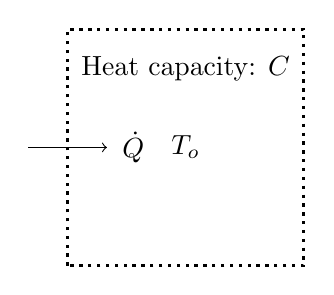
\begin{tikzpicture}
\draw[dotted,very thick]  (-1.5,-1.5) rectangle (1.5,1.5);
\draw (0,0) node {$T_{o}$};
\draw (0,1) node {Heat capacity: $C$};
\draw[->] (-2,0) -- ++(1,0) node[right=2pt] {$\dot{Q}$}; 
\end{tikzpicture} 
& 
%--------- Thermal Convection ''Heat Flow''
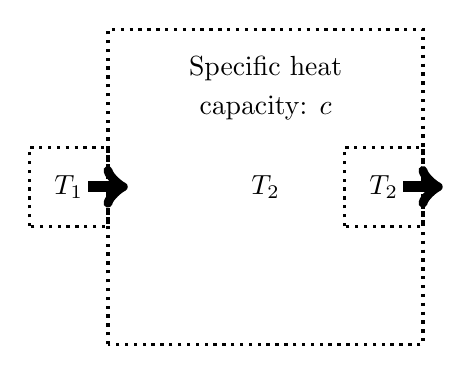
\begin{tikzpicture}
\draw[dotted,very thick]  (-2,-2) rectangle (2,2);
\draw[dotted,very thick]  (-3,-0.5) rectangle ++(1,1);
\draw[dotted,very thick]  (1,-0.5) rectangle ++(1,1);
\draw (0,1.5) node {Specific heat};
\draw (0,1.0) node {capacity: $c$};
\draw (0,0) node {$T_{2}$};
\draw (-2.5,0) node {$T_{1}$};
\draw (1.5,0) node {$T_{2}$};
\draw[->,line width=4pt] (-2.25,0) -- ++(.5,0);
\draw[->,line width=4pt] (1.75,0) -- ++(.5,0);
 \end{tikzpicture}  
 \\\hline

\rule[-8pt]{0pt}{0pt}\rule{0pt}{14pt}  
Component law & 		$T = \dot{Q}R$ & 
							$\dot{Q} = C \frac{dT_o}{dt}$ & 
							$\dot{Q} = \dot{m} c T$ \\\hline
							
\rule[-8pt]{0pt}{0pt}\rule{0pt}{14pt}							
Laplace Transform &	$T(s)=\dot{Q}(s)R$ & 
							$\dot{Q}(s)=CsT_o(s)$ & 
							$\dot{Q}(s)=\dot{m}cT(s)$ \\\hline

 							 
Impedance Component  &  
 %--------- Thermal resistance model
 \begin{tikzpicture}
\draw (5,0) node[inner sep=0,outer sep=0] (C) {\input{../DrawingElements/CircuitElements/resistor.tex}};
\draw (C) node[above=12pt] {$R$};
\draw[->] (C.0) ++(.1,0) -- node[pos=.5,below=2pt] {$\dot{Q}$} ++(.5,0);
\draw[<-] (C.180) ++(-.1,0) -- node[pos=.5,below=2pt] {$\dot{Q}$} ++(-.5,0);
\draw (C.0) node[draw,fill,inner sep=0pt,outer sep=0pt,circle] {$\rule{2pt}{0pt}$};
\draw (C.0) node[above=4pt] {$T_{2}$};
\draw (C.180) node[draw,fill,inner sep=0pt,outer sep=0pt,circle] {$\rule{2pt}{0pt}$};
\draw (C.180) node[above=4pt] {$T_{1}$};
%\draw (C) ++(0,-1) node {$\dot{Q}R = T_{1} - T_{2}$};
\draw (C) ++(0,-1) node {$T = T_{1} - T_{2}$};
\end{tikzpicture} 
& 
%--------- Thermal capacitor model
 \begin{tikzpicture} 
\draw (5,0) node[inner sep=0,outer sep=0,rotate=90] (C) {\input{../DrawingElements/CircuitElements/capacitor.tex}};
\draw (C) node[right=12pt] {$\frac{1}{Cs}$};
\draw[->] (C.0) ++(.3,0) -- node[pos=0,right=2pt] {$\dot{Q}$} ++(0,-.5);
\draw (C.0) node[draw,fill,inner sep=0pt,outer sep=0pt,circle] {$\rule{2pt}{0pt}$};
\draw (C.0) node[above=4pt] {$T_{o}$};
\draw (C.180) node[draw,fill,inner sep=0pt,outer sep=0pt,circle] {$\rule{2pt}{0pt}$};
\draw (C.180) node[below=4pt] {$T_{ref}=0$}; 
\end{tikzpicture} 
& 
 \begin{tikzpicture} 
\draw (7,0) node (C) {\input{../DrawingElements/CircuitElements/resistor.tex}};
\draw (5,0) node[isosceles triangle,draw,very thick,inner sep=2pt] (G) {$1$};
\draw (C) node[above=12pt] {$R=\frac{1}{c\dot{m}}$};
\draw[very thick] (G.180) ++(-.75,0) node[draw,fill,inner sep=0pt,outer sep=0pt,circle] (Gin) {$\rule{2pt}{0pt}$} -- (G.180);
\draw (Gin) node[above=4pt] {$T_{1}$};
\draw[<-] (Gin) ++(-.1,0) -- node[pos=-1.5,below left=2pt] {$\dot{Q}_{in}=0$} ++(-.5,0);
\draw[very thick] (G.0) ++(-0.1,0) --   ++(0.8,0) ;
\draw[very thick] (C.0) ++(-0.2,0) -- ++(.5,0) node (C_p) {} node[above=4pt]  {$T_{2}$};
\draw (C_p.0)++(-0.1,0) node[draw,fill,inner sep=0pt,outer sep=0pt,circle] {$\rule{2pt}{0pt}$};
\draw[->] (C_p.0) ++(.1,0) -- node[pos=-.5,below right=2pt] {$\dot{Q}$} ++(.5,0);
\draw (C) ++(0,-1) node {$T = T_{1} - T_{2}$};
\end{tikzpicture}

\end{tabular}
\end{center}
\end{frame}


%%%%%%%%%%%%%%%%%%%%%%%%%%%%%%%%%%%
\begin{frame}{DC Motor}
\begin{center}
\begin{tabular}{c|c}
   &   DC motor \\\hline
   
Component & 
\begin{tikzpicture}[scale=1.3,inner sep=0pt,outer sep=0pt,very thick]
\draw (0,0) node[fill=black] (a) {}; 
\draw (3.5,0) node[fill=black] (c) {};
\draw (0,-2) node[fill=black] (d) {};
\draw (2,-2) node[fill=black] (e) {};
\draw (3.5,-2) node[fill=black] (f) {};
 
\draw (1,0) node (R1) {\input{../DrawingElements/CircuitElements/resistor.tex}};
\draw (1,0) node[above=.2in] {$R_{a}$};
\draw (2.5,0) node (L1) {\input{../DrawingElements/CircuitElements/inductor.tex}};
\draw (2.5,0) node[above=.2in] {$L_{a}$};
\draw (3.5,-1) node (Rot) {\input{../DrawingElements/CircuitElements/rotor.tex}}; 
\draw[->] (4,-1) ++(0,.5)  node[above=2pt] {$\theta$}  .. controls  ++(-.15,-.3) and ++(-.15,.3) ..  ++(0,-1);
\draw[->] (4.25,-1) ++(0,.5) node[above=2pt] {$\tau_{m}$}  .. controls  ++(-.15,-.3) and ++(-.15,.3) ..  ++(0,-1);
\draw[->] (3.35,-.1) -- node[left=1pt] {$i_{a}$} ++(0,-.5); 
\draw (3.5,-1) node[left=.2in] {$\begin{matrix} + \\ v_{b} \\ -\end{matrix}$};
\draw (0,-1) node (V) {\input{../DrawingElements/CircuitElements/voltagesource.tex}};
\draw (0,-1) node[left=.2in]{$v_{a}$};
\draw (a) -- (R1);
\draw (R1) -- (L1);
\draw (L1) -| (Rot);
\draw (Rot) -- (f);
\draw (f) -- (d);
\draw (a) -- (V);
\draw (d) -- (V);


\end{tikzpicture}
 \\\hline
 
 						 
Component Law &  	
\pbox{10cm}
{$v_{b} = K_{e}\dot{\theta}$ \\ 
$\tau_{m} = K_{t} i_{a}$ \\ 
$v_a(t) = i_a(t)R + L\frac{di_a(t)}{dt} + v_b(t)$ }

\\\hline
 							 
Block Diagram  &  
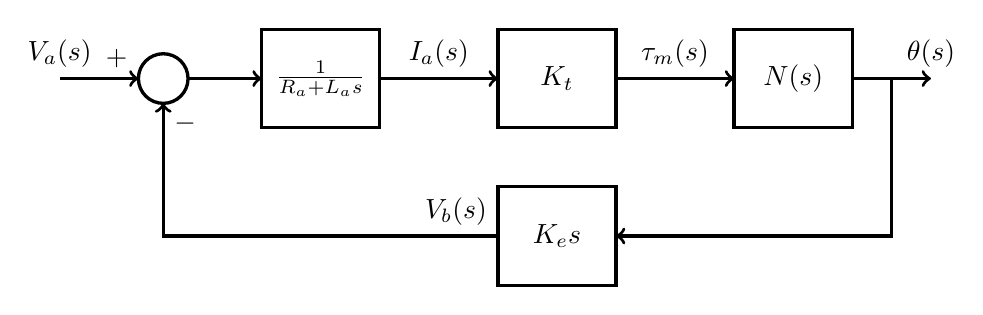
\begin{tikzpicture}[inner sep=0pt,outer sep=0pt,very thick,
sysblock/.style={draw,rectangle,inner sep=2pt,minimum width=1.5cm,minimum height=1.25cm,very thick}]
\draw (0,0) node[draw,circle] (sum) {$\rule{0pt}{18pt}$};
\draw (2,0) node[sysblock] (a) {$\frac{1}{R_{a} + L_{a}s}$};
\draw (5,0) node[sysblock] (b) {$K_{t}$};
\draw (8,0) node[sysblock] (c) {$N(s)$};
\draw (5,-2) node[sysblock] (d) {$K_{e}s$};
\draw[<-] (sum.180) node[above left=4pt] {$+$} -- ++(-1,0) node[above=4pt] {$V_{a}(s)$};
\draw[->] (sum.0) -- (a.180);
\draw[->] (a.0) -- node[pos=.5,above=4pt] {$I_{a}(s)$} (b.180);
\draw[->] (b.0) -- node[pos=.5,above=4pt] {$\tau_{m}(s)$} (c.180);
\draw[->] (c.0) -- ++(1,0) node[above=4pt] {$\theta(s)$};
\draw[->] (c.0) -- ++(.5,0) |- (d.0);
\draw[->] (d.180) node[above left=4pt] {$V_{b}(s)$} -| (sum.-90) node[below right=4pt] {$-$};
\end{tikzpicture}  
\end{tabular}
\end{center}
\end{frame}


%%%%%%%%%%%%%%%%%%%%%%%%%%%%%%%%%%%
\pagebreak
\begin{frame}{Hydraulic}
\begin{center}
\begin{tabular}{c|c}
   &   Hydraulic \\\hline

Component &    
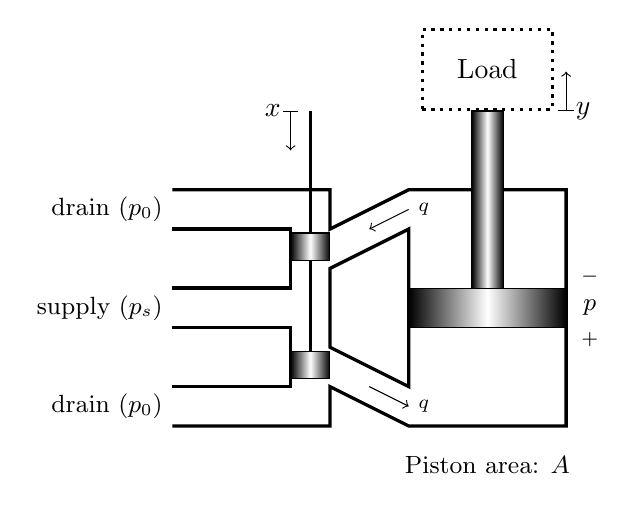
\begin{tikzpicture}
% tank
\draw[very thick] (0,0) -- ++(2,0) -- ++(0,-.5) -- ++(1,.5) -- ++(2,0) -- ++(0,-3) -- ++(-2,0) -- ++(-1,.5) -- ++(0,-.5) -- ++(-2,0);
\draw[very thick] (0,-.5) -- ++(1.5,0) -- ++(0,-.75) -- ++(-1.5,0);
\draw[very thick] (0,-1.75) -- ++(1.5,0) -- ++(0,-.75) -- ++(-1.5,0);
\draw[very thick] (2,-1) -- ++(1,.5) -- ++(0,-2) -- ++(-1,.5) -- cycle;
\draw (4,-3.5) node {\small Piston area: $A$};
\draw (0,-.25) node[left] {\small drain ($p_{0}$)};
\draw (0,-1.5) node[left] {\small supply ($p_{s}$)};
\draw (0,-2.75) node[left] {\small drain ($p_{0}$)};
\draw[->] (3,-.25) node[right] {\scriptsize$q$} -- ++(-.5,-.25);
\draw[->] (2.5,-2.5) -- ++(.5,-.25)  node[right] {\scriptsize$q$};
\draw (5.3,-1.9) node {\scriptsize $+$} ++(0,.4) node{\small $p$} ++(0,.4) node {\scriptsize$-$};

% valves
\draw[very thick,color=black] (1.75,-2.1) -- ++(0,3.1);
\draw[fill,left color=black,right color=black,middle color=white] (1.5,-.9) rectangle ++(.5,.35);
\draw[fill,left color=black,right color=black,middle color=white] (1.5,-2.4) rectangle ++(.5,.35);
\draw[|->] (1.5,1) node[left] {$x$} -- ++(0,-.5); 

% piston
\draw[fill,left color=black,right color=black,middle color=white] (4,-1.5) ++(-.2,0) rectangle ++(.4,2.5);
\draw[fill,left color=black,right color=black,middle color=white] (3,-1.75) rectangle ++(2,.5);
\draw[|->] (5,1) node[right] {$y$} -- ++(0,.5);

% load
\draw (4,1) node[draw,very thick,above,dotted,rectangle,minimum width=.65in,minimum height=.4in] {Load};
\end{tikzpicture}
\\\hline

\rule[-8pt]{0pt}{0pt}
Component Law &  
\pbox{10cm}
{$\delta q = k_x\delta x - k_p \delta p$ \\
$f = p A $ \\
$y = \frac{1}{A} \int q dt $ }

\\\hline

Block Diagram & 
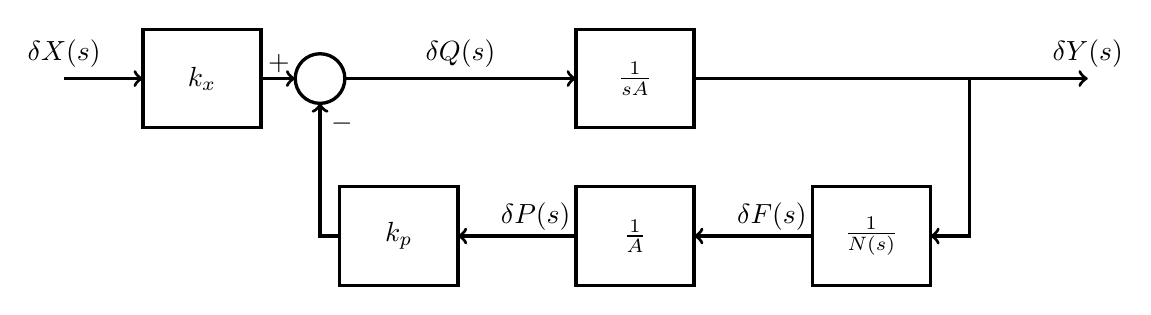
\begin{tikzpicture}[inner sep=0pt,outer sep=0pt,very thick,
sysblock/.style={draw,rectangle,inner sep=2pt,minimum width=1.5cm,minimum height=1.25cm,very thick}]
\draw (-1.5,0) node[sysblock] (d) {$k_{x}$};
\draw (0,0) node[draw,circle] (sum) {$\rule{0pt}{18pt}$};
\draw (4,0) node[sysblock] (a) {$\frac{1}{sA}$};
\draw (4,-2) node[sysblock] (b) {$\frac{1}{A}$};
\draw (7,-2) node[sysblock] (b1) {$\frac{1}{N(s)}$};
\draw (1,-2) node[sysblock] (c) {$k_{p}$};
\draw[<-] (d.180)  -- ++(-1,0) node[above=4pt] {$\delta X(s)$};
\draw[->] (d.0) -- (sum.180) node[above left=2pt] {$+$};
\draw[->] (sum.0) -- node[pos=.5,above=4pt] {$\delta Q(s)$} (a.180);
\draw[->] (a.0) -- ++(5,0) node[above=4pt] {$\delta Y(s)$};
\draw[->] (a.0) -- ++(3.5,0) |- (b1.0);
\draw[->] (b1.180) node[above left=2pt] {$\delta F(s)$} -- (b.0);
\draw[->] (b.180) node[above left=2pt] {$\delta P(s)$} -- (c.0);
\draw[->] (c.180)  -| (sum.-90) node[below right=4pt] {$-$};

\end{tikzpicture}





\end{tabular}
\end{center}
\end{frame}

\end{document}


};
\draw (k) node[above=6pt] {$\frac{1}{k}$};
\draw (3,-1) node[rotate=90] (J2) {\documentclass[12pt]{article}
% \newcommand{\mainfolder}{/Users/coulston/Dropbox/EENG307Current}  	                    % @ Work PC
%\newcommand{\mainfolder}{C:/Users/Chris/Dropbox/Mycourses/EENG307Current}  	% @ Work Laptop
\newcommand{\mainfolder}{C:/Users/chris/Dropbox/Mycourses/EENG307Current}		% @ Home PC

% \newcommand{\mainfolder}{$HOME/Dropbox/EENG307Current}
\newcommand{\commonmaterial}{\mainfolder/CommonMaterial}
\input{\mainfolder/Headers/packageheader}
\input{\mainfolder/Headers/coursedefheader}

\usepackage{pbox}
%\usepackage{siunitx}
%\usepackage{draftwatermark}
%\SetWatermarkText{DRAFT}
%\SetWatermarkScale{1}

\setlength{\topmargin}{-.75in}
\setlength{\textheight}{9.25in}
\setlength{\oddsidemargin}{-0.25in}
\setlength{\evensidemargin}{-0.25in}
\setlength{\textwidth}{7in}




\begin{document}



%%%%%%%%%%%%%%%%%%%%%%%%%%%%%%%%%%%
\begin{frame}{Electrical Impedance}%
\begin{center}%
\mode<article>{

\begin{tabular}{c|ccc}
 & resistor & capacitor & inductor  \\\hline
 Component & \input{./figures/resistor.tex} & \input{./figures/capacitor.tex} & \input{./figures/inductor.tex}\\\hline
\rule[-8pt]{0pt}{0pt}\rule{0pt}{14pt} 
Component law & $v_1-v_2=iR$ & $i = C\frac{d(v_1-v_2)}{dt}$ & $v_1-v_2=L\frac{di}{dt}$  \\\hline
\rule[-8pt]{0pt}{0pt}\rule{0pt}{14pt} 
Laplace Transform & $V(s)= I(s)R$ & $V(s) = \frac{1}{Cs}I(s)$ & $V(s) = LsI(s)$ \\\hline
Impedance Component & \input{./figures/resistorimpedance.tex} & \input{./figures/capacitorimpedance.tex} & \input{./figures/inductorimpedance.tex}

\end{tabular}}
\end{center}
\end{frame}


%%%%%%%%%%%%%%%%%%%%%%%%%%%%%%%%%%%
\begin{frame}{Fluid Impedance}
\graphicspath{}
\begin{center}
\mode<article>{

\begin{tabular}{c|cc}
 & valve & tank \\\hline
%Component &\begin{tikzpicture}
\draw (.75,0) node (valve) {\input{\mainfolder/DrawingElements/FluidElements/valve.tex}};
\draw (.75,0) node[above=9pt] {$R$};
\draw (-.2,.25) node[above] {$p_{1}$};
\draw[<-] (valve.180) --  ++(-.5,0) node[left] {$q$};
\draw[->] (valve.0) -- ++(.5,0)  node[right] {$q$};
\draw (1.7,.25) node[above] {$p_{2}$};
\draw (.75,1.5) node {$p = p_{1}-p_{2}$};
\end{tikzpicture} &  \input{./figures/figurestank2.tex} \\\hline
Component &\begin{tikzpicture}
\draw (.75,0) node (valve) {\input{\mainfolder/DrawingElements/FluidElements/valve.tex}};
\draw (.75,0) node[above=9pt] {$R$};
\draw (-.2,.25) node[above] {$p_{1}$};
\draw[<-] (valve.180) --  ++(-.5,0) node[left] {$q$};
\draw[->] (valve.0) -- ++(.5,0)  node[right] {$q$};
\draw (1.7,.25) node[above] {$p_{2}$};
\draw (.75,1.5) node {$p = p_{1}-p_{2}$};
\end{tikzpicture} &  \input{./figures/tank.tex} \\\hline
\rule[-8pt]{0pt}{0pt}\rule{0pt}{14pt} Component law & $p=Rq$ & $\frac{A}{\rho g}\frac{dp}{dt} = q_{1} - q_{2}$ \\\hline
\rule[-8pt]{0pt}{0pt}\rule{0pt}{14pt} Laplace Transform & $P(s)= RQ(s)$ & $\frac{A}{\rho g}sP(s) = Q_{1}(s)-Q_{2}(s)$ \\\hline
 Impedance Component & \input{./figures/valveanalogycopy.tex} & \input{./figures/tankanalogycopy.tex}
 \end{tabular}}
 
\mode<presentation>{\resizebox{11cm}{!}{

\begin{tabular}{c|cc}
 & valve & tank \\\hline
Component &\begin{tikzpicture}
\draw (.75,0) node (valve) {\input{\mainfolder/DrawingElements/FluidElements/valve.tex}};
\draw (.75,0) node[above=9pt] {$R$};
\draw (-.2,.25) node[above] {$p_{1}$};
\draw[<-] (valve.180) --  ++(-.5,0) node[left] {$q$};
\draw[->] (valve.0) -- ++(.5,0)  node[right] {$q$};
\draw (1.7,.25) node[above] {$p_{2}$};
\draw (.75,1.5) node {$p = p_{1}-p_{2}$};
\end{tikzpicture} & \input{./figures/tank2.tex} \\\hline
\rule[-8pt]{0pt}{0pt}\rule{0pt}{14pt} Component law & $p=Rq$ & $\frac{A}{\rho g}\frac{dp}{dt} = q_{1} - q_{2}$ \\\hline
\rule[-8pt]{0pt}{0pt}\rule{0pt}{14pt} Laplace Transform & $P(s)= RQ(s)$ & $\frac{A}{\rho g}sP(s) = Q_{1}(s)-Q_{2}(s)$ \\\hline
 Impedance Component & \input{./figures/valveanalogycopy.tex} & \input{./figures/tankanalogycopy.tex}
 \end{tabular}}}
\end{center}
\end{frame}

\pagebreak

%%%%%%%%%%%%%%%%%%%%%%%%%%%%%%%%%%%
\begin{frame}{Mechanical Impedance}%
\begin{center}%
\mode<article>{\begin{tabular}{c|ccc}
 & mass & spring & damper \\\hline
 Component & \begin{tikzpicture}
%  \draw(-1,2.5) node (text) {\textsf{fixed point}};
%   \draw[->] (text.180) -- ++(-.7,0);
   \draw[inner sep=0pt,outer sep=0pt,very thick] (-3,1) node (gnd1) {\input{\mainfolder/DrawingElements/MechanicalElements/ground.tex}};
   \draw[->|,dotted] (-3,1.75) -- node[pos=.5,above] {$x_{f}$} ++(3.6,0); 
    \draw[very thick] (0,0) rectangle (1.2,1);
    \draw (.6,.5) node {$m$};
    \draw[->,thick] (1.2,.5) -- ++(.5,0) node[right] {$f$};
    \draw[|->,thick] (.6,1.2) node[above=2pt] {$x$} -- ++(.5,0);  
\end{tikzpicture}
 & \begin{tikzpicture}
\draw (.75,0) node[inner sep=0,outer sep=0] (K1) {\input{\mainfolder/DrawingElements/MechanicalElements/spring.tex}};
\draw (K1)  node[above=6pt] {$k$};
\draw[very thick] (K1.180) -- ++(-.2,0);
\draw[very thick] (K1.0) -- ++(0.2,0);
\draw[<-,thick] (K1.0) ++(.2,0) -- ++(.5,0) node[right] {$f$};
\draw[<-,thick] (K1.180) ++(-.2,0) -- ++(-.5,0) node[left] {$f$};
\draw[|->,thick] (K1.180) ++(-.2,.4) node[above=2pt] {$x_{1}$} -- ++(.5,0);  
\draw[|->,thick] (K1.0) ++(.2,.4) node[above=2pt] {$x_{2}$} -- ++(.5,0);  
\draw<2-> (K1) ++(0,-.6) node {$f=k(x_{1}-x_{2})$};
\end{tikzpicture}
 & \begin{tikzpicture}
\draw[very thick] (-.2,0) -- (0,0);
\draw (.75,0) node {\input{\mainfolder/DrawingElements/MechanicalElements/damper.tex}};
\draw (.75,0) node[above=9pt] {$b$};
\draw[very thick] (1.5,0) -- ++(.2,0);
    \draw[<-,thick] (1.5,0) ++(.2,0) -- ++(.5,0) node[right] {$f$};
    \draw[<-,thick] (-.2,0) -- ++(-.5,0) node[left] {$f$};
    \draw[|->,thick] (-.2,.4) node[above=2pt] {$x_{1}$} -- ++(.5,0);  
    \draw[|->,thick] (1.7,.4) node[above=2pt] {$x_{2}$} -- ++(.5,0);  
    \draw (.6,-.6) node {$x=x_{1}-x_{2}$};
  %  \draw (.6,-1.2) node {$f=b\dot{x}$};
\end{tikzpicture}\\\hline
\rule[-8pt]{0pt}{0pt}\rule{0pt}{14pt} 
Component law & $f = m\ddot{x}$ & $f = kx$ & $f=b\dot{x}$  \\\hline
\rule[-8pt]{0pt}{0pt}\rule{0pt}{14pt} Laplace Transform & $X(s)= \frac{1}{ms^{2}}F(s)$ & $X(s) = \frac{1}{k}F(s)$ & $X(s) = \frac{1}{bs}F(s)$ \\\hline
\begin{minipage}[b]{1.5in}\begin{center}Impedance Component \\
(positive $f$ direction agrees with positive $x$ direction)\end{center}
\end{minipage}
& \input{figures/massimpedance.tex} & \input{figures/springimpedance.tex} & \input{figures/damperimpedance.tex}
 \end{tabular}}
\mode<presentation>{\resizebox{10cm}{!}{\begin{tabular}{c|ccc}
 & mass & spring & damper \\\hline
 Component & \begin{tikzpicture}
%  \draw(-1,2.5) node (text) {\textsf{fixed point}};
%   \draw[->] (text.180) -- ++(-.7,0);
   \draw[inner sep=0pt,outer sep=0pt,very thick] (-3,1) node (gnd1) {\input{\mainfolder/DrawingElements/MechanicalElements/ground.tex}};
   \draw[->|,dotted] (-3,1.75) -- node[pos=.5,above] {$x_{f}$} ++(3.6,0); 
    \draw[very thick] (0,0) rectangle (1.2,1);
    \draw (.6,.5) node {$m$};
    \draw[->,thick] (1.2,.5) -- ++(.5,0) node[right] {$f$};
    \draw[|->,thick] (.6,1.2) node[above=2pt] {$x$} -- ++(.5,0);  
\end{tikzpicture}
& \begin{tikzpicture}
\draw (.75,0) node[inner sep=0,outer sep=0] (K1) {\input{\mainfolder/DrawingElements/MechanicalElements/spring.tex}};
\draw (K1)  node[above=6pt] {$k$};
\draw[very thick] (K1.180) -- ++(-.2,0);
\draw[very thick] (K1.0) -- ++(0.2,0);
\draw[<-,thick] (K1.0) ++(.2,0) -- ++(.5,0) node[right] {$f$};
\draw[<-,thick] (K1.180) ++(-.2,0) -- ++(-.5,0) node[left] {$f$};
\draw[|->,thick] (K1.180) ++(-.2,.4) node[above=2pt] {$x_{1}$} -- ++(.5,0);  
\draw[|->,thick] (K1.0) ++(.2,.4) node[above=2pt] {$x_{2}$} -- ++(.5,0);  
\draw<2-> (K1) ++(0,-.6) node {$f=k(x_{1}-x_{2})$};
\end{tikzpicture}
 & \begin{tikzpicture}
\draw[very thick] (-.2,0) -- (0,0);
\draw (.75,0) node {\input{\mainfolder/DrawingElements/MechanicalElements/damper.tex}};
\draw (.75,0) node[above=9pt] {$b$};
\draw[very thick] (1.5,0) -- ++(.2,0);
    \draw[<-,thick] (1.5,0) ++(.2,0) -- ++(.5,0) node[right] {$f$};
    \draw[<-,thick] (-.2,0) -- ++(-.5,0) node[left] {$f$};
    \draw[|->,thick] (-.2,.4) node[above=2pt] {$x_{1}$} -- ++(.5,0);  
    \draw[|->,thick] (1.7,.4) node[above=2pt] {$x_{2}$} -- ++(.5,0);  
    \draw (.6,-.6) node {$x=x_{1}-x_{2}$};
  %  \draw (.6,-1.2) node {$f=b\dot{x}$};
\end{tikzpicture}\\\hline
\rule{0pt}{14pt} Component law & $M\ddot{x}=f$ & $f = kx$ & $f=b\dot{x}$  \\\hline
\rule[-8pt]{0pt}{0pt}\rule{0pt}{14pt} Laplace Transform & $X(s)= \frac{1}{Ms^{2}}F(s)$ & $X(s) = \frac{1}{k}F(s)$ & $X(s) = \frac{1}{bs}F(s)$ \\\hline
\begin{minipage}[b]{1.5in}\begin{center}Impedance Component \\
(positive $f$ direction agrees with positive $x$ direction)\end{center}
\end{minipage}
& \input{./figures/massimpedance.tex} & \input{./figures/springimpedance.tex} & \input{./figures/damperimpedance.tex}
 \end{tabular}}}
\end{center}
\end{frame}


%%%%%%%%%%%%%%%%%%%%%%%%%%%%%%%%%%%
\begin{frame}{Rotational Impedance}
\begin{center}
\mode<article>{\begin{tabular}{c|ccc}
 & mass & spring & damper \\\hline
 Component & \begin{minipage}[b]{.75in}\begin{tikzpicture}
    \draw[very thick] (.5,0) node[cylinder,draw,shape aspect=.55,minimum width=1cm,minimum height=1.5cm] (J) {$J$};
    \draw[->] (-.2,.5) node[above] {$\theta$}  .. controls  ++(-.15,-.3) and ++(-.15,.3) ..  ++(0,-1);
    \draw[->] (1.4,-.5) node[below] {$\tau$}  .. controls  ++(.15,.3) and ++(.15,-.3) ..  ++(0,1);
    \draw (.5,-1) node {$J\ddot{\theta}=\tau$};
\end{tikzpicture}\\\vspace{.1in}\end{minipage} & \begin{tikzpicture}
\draw[very thick] (-.2,0) -- (0,0);
\draw (.75,0) node {\input{\mainfolder/DrawingElements/MechanicalElements/spring.tex}};
\draw[very  thick] (1.5,0) -- ++(.2,0);
\draw (.75,0) node[above=9pt] {$k$};
\draw[->] (-.2,.5) node[above] {$\theta_{1}$}  .. controls  ++(-.15,-.3) and ++(-.15,.3) ..  ++(0,-1);
\draw[->] (-.5,.5) node[above] {$\tau$}  .. controls  ++(-.15,-.3) and ++(-.15,.3) ..  ++(0,-1);
\draw[->] (1.5,.5) node[above] {$\theta_{2}$}  .. controls  ++(-.15,-.3) and ++(-.15,.3) ..  ++(0,-1);
\draw[->] (1.9,.5) node[above] {$\tau$}  .. controls  ++(.15,-.3) and ++(.15,.3) ..  ++(0,-1);
\draw (.5,-1) node {$\theta=\theta_{1} - \theta_{2}$};
\end{tikzpicture} & \begin{tikzpicture}
\draw[very thick] (-.2,0) -- (0,0);
\draw (.75,0) node {\input{\mainfolder/DrawingElements/MechanicalElements/damper.tex}};
\draw[very  thick] (1.5,0) -- ++(.2,0);
\draw (.75,0) node[above=9pt] {$b$};
\draw[->] (-.2,.5) node[above] {$\theta_{1}$}  .. controls  ++(-.15,-.3) and ++(-.15,.3) ..  ++(0,-1);
\draw[->] (-.5,.5) node[above] {$\tau$}  .. controls  ++(-.15,-.3) and ++(-.15,.3) ..  ++(0,-1);
\draw[->] (1.5,.5) node[above] {$\theta_{2}$}  .. controls  ++(-.15,-.3) and ++(-.15,.3) ..  ++(0,-1);
\draw[->] (1.9,.5) node[above] {$\tau$}  .. controls  ++(.15,-.3) and ++(.15,.3) ..  ++(0,-1);
\draw (.5,-1) node {$\dot{\theta}=\dot{\theta}_{1} - \dot{\theta}_{2}$};
\end{tikzpicture}\\\hline
 \rule[-8pt]{0pt}{0pt}\rule{0pt}{12pt} 
 Component Law & $\tau = J\ddot{\theta}$ & $\tau = k\theta$ & $\tau = b\dot{\theta}$ \\\hline
\rule[-8pt]{0pt}{0pt}\rule{0pt}{14pt} Laplace Transform & $\theta(s)= \frac{1}{Js^{2}}\tau(s)$ & $\theta(s) = \frac{1}{k}\tau(s)$ & $\theta(s) = \frac{1}{bs}\tau(s)$ \\\hline
\begin{minipage}[b]{1.5in}\begin{center}Impedance Component
\end{center}
\end{minipage}
& \begin{tikzpicture}
\draw (0,0) node (R) {\begin{tikzpicture}
\draw (0,0) node[circle,fill,inner sep=1pt,] {} node[above] {$\theta$};
\draw[very thick] (0,0)  -- ++(0,-.37);
\draw[very thick] (0,-1) node[rectangle,draw,minimum width=.1in,minimum height=.5in] {};
\draw[very thick] (0,-1.65) -- ++(0,-.37);
\draw[very thick] (0,-2) node{\input{\mainfolder/DrawingElements/CircuitElements/elground.tex}};
\end{tikzpicture}
};

\draw (R) node[right=6pt] {$\frac{1}{Js^{2}}$};
%\draw (6.1,.75) node[above] {$+$};
\draw (1,0) node[right] {$\begin{matrix} + \\ \\ \theta(s)\\  \\ - \end{matrix}$};
%\draw (7.9,.75) node[above] {$-$};
\draw[->] (-.3,.5) -- node[pos=.5,left] {$\tau(s)$} ++(0,-1);  

\end{tikzpicture} & \begin{tikzpicture}
\draw (7,.2) node (R) {\begin{tikzpicture}
\draw (0,0) node[circle,fill,inner sep=1pt,] {} node[above] {$\theta_{1}$};
\draw[very thick] (0,0) -- ++(.37,0);
\draw[very thick] (1,0) node[rectangle,draw,minimum width=.5in,minimum height=.1in] {};
\draw[very thick] (1.65,0) -- ++(.37,0);
\draw (2.02,0) node[circle,fill,inner sep=1pt,] {} node[above] {$\theta_{2}$};
\end{tikzpicture}
};
\draw (R) node[above=1pt] {$\frac{1}{k}$};
%\draw (6.1,.75) node[above] {$+$};
%\draw (7,.75) node[above] {$X(s)$};
%\draw (7.9,.75) node[above] {$-$};
\draw[->] (6.5,-.3) -- node[pos=.5,below] {$\tau(s)$} ++(1,0);  
\draw (7,-1.5) node[above] {$\begin{matrix} + & \theta(s) & - \end{matrix}$};

\end{tikzpicture} & \input{./figures/rotdamperimpedance.tex}
 \end{tabular}}
\mode<presentation>{\resizebox{10cm}{!}{\begin{tabular}{c|ccc}
 & mass & spring & damper \\\hline
 Component & \begin{tikzpicture}
    \draw[very thick] (.5,0) node[cylinder,draw,shape aspect=.55,minimum width=1cm,minimum height=1.5cm] (J) {$J$};
    \draw[->] (-.2,.5) node[above] {$\theta$}  .. controls  ++(-.15,-.3) and ++(-.15,.3) ..  ++(0,-1);
    \draw[->] (1.4,-.5) node[below] {$\tau$}  .. controls  ++(.15,.3) and ++(.15,-.3) ..  ++(0,1);
    \draw (.5,-1) node {$J\ddot{\theta}=\tau$};
\end{tikzpicture} & \begin{tikzpicture}
\draw[very thick] (-.2,0) -- (0,0);
\draw (.75,0) node {\input{\mainfolder/DrawingElements/MechanicalElements/spring.tex}};
\draw[very  thick] (1.5,0) -- ++(.2,0);
\draw (.75,0) node[above=9pt] {$k$};
\draw[->] (-.2,.5) node[above] {$\theta_{1}$}  .. controls  ++(-.15,-.3) and ++(-.15,.3) ..  ++(0,-1);
\draw[->] (-.5,.5) node[above] {$\tau$}  .. controls  ++(-.15,-.3) and ++(-.15,.3) ..  ++(0,-1);
\draw[->] (1.5,.5) node[above] {$\theta_{2}$}  .. controls  ++(-.15,-.3) and ++(-.15,.3) ..  ++(0,-1);
\draw[->] (1.9,.5) node[above] {$\tau$}  .. controls  ++(.15,-.3) and ++(.15,.3) ..  ++(0,-1);
\draw (.5,-1) node {$\theta=\theta_{1} - \theta_{2}$};
\end{tikzpicture} & \begin{tikzpicture}
\draw[very thick] (-.2,0) -- (0,0);
\draw (.75,0) node {\input{\mainfolder/DrawingElements/MechanicalElements/damper.tex}};
\draw[very  thick] (1.5,0) -- ++(.2,0);
\draw (.75,0) node[above=9pt] {$b$};
\draw[->] (-.2,.5) node[above] {$\theta_{1}$}  .. controls  ++(-.15,-.3) and ++(-.15,.3) ..  ++(0,-1);
\draw[->] (-.5,.5) node[above] {$\tau$}  .. controls  ++(-.15,-.3) and ++(-.15,.3) ..  ++(0,-1);
\draw[->] (1.5,.5) node[above] {$\theta_{2}$}  .. controls  ++(-.15,-.3) and ++(-.15,.3) ..  ++(0,-1);
\draw[->] (1.9,.5) node[above] {$\tau$}  .. controls  ++(.15,-.3) and ++(.15,.3) ..  ++(0,-1);
\draw (.5,-1) node {$\dot{\theta}=\dot{\theta}_{1} - \dot{\theta}_{2}$};
\end{tikzpicture}\\\hline
\rule[-8pt]{0pt}{0pt}\rule{0pt}{14pt} Laplace Transform & $\theta(s)= \frac{1}{Js^{2}}\tau(s)$ & $\theta(s) = \frac{1}{k}\tau(s)$ & $\theta(s) = \frac{1}{bs}\tau(s)$ \\\hline
\begin{minipage}[b]{1.5in}\begin{center}Impedance Component 
\end{center}
\end{minipage}
& \begin{tikzpicture}
\draw (0,0) node (R) {\begin{tikzpicture}
\draw (0,0) node[circle,fill,inner sep=1pt,] {} node[above] {$\theta$};
\draw[very thick] (0,0)  -- ++(0,-.37);
\draw[very thick] (0,-1) node[rectangle,draw,minimum width=.1in,minimum height=.5in] {};
\draw[very thick] (0,-1.65) -- ++(0,-.37);
\draw[very thick] (0,-2) node{\input{\mainfolder/DrawingElements/CircuitElements/elground.tex}};
\end{tikzpicture}
};

\draw (R) node[right=6pt] {$\frac{1}{Js^{2}}$};
%\draw (6.1,.75) node[above] {$+$};
\draw (1,0) node[right] {$\begin{matrix} + \\ \\ \theta(s)\\  \\ - \end{matrix}$};
%\draw (7.9,.75) node[above] {$-$};
\draw[->] (-.3,.5) -- node[pos=.5,left] {$\tau(s)$} ++(0,-1);  

\end{tikzpicture} & \begin{tikzpicture}
\draw (7,.2) node (R) {\begin{tikzpicture}
\draw (0,0) node[circle,fill,inner sep=1pt,] {} node[above] {$\theta_{1}$};
\draw[very thick] (0,0) -- ++(.37,0);
\draw[very thick] (1,0) node[rectangle,draw,minimum width=.5in,minimum height=.1in] {};
\draw[very thick] (1.65,0) -- ++(.37,0);
\draw (2.02,0) node[circle,fill,inner sep=1pt,] {} node[above] {$\theta_{2}$};
\end{tikzpicture}
};
\draw (R) node[above=1pt] {$\frac{1}{k}$};
%\draw (6.1,.75) node[above] {$+$};
%\draw (7,.75) node[above] {$X(s)$};
%\draw (7.9,.75) node[above] {$-$};
\draw[->] (6.5,-.3) -- node[pos=.5,below] {$\tau(s)$} ++(1,0);  
\draw (7,-1.5) node[above] {$\begin{matrix} + & \theta(s) & - \end{matrix}$};

\end{tikzpicture} & \input{./figures/rotdamperimpedance.tex}
 \end{tabular}}}
\end{center}
\end{frame}


\pagebreak

%%%%%%%%%%%%%%%%%%%%%%%%%%%%%%%%%%%
\begin{frame}{Thermal Impedance}
\begin{center}
\begin{tabular}{c|ccc}
 & Resistance & Capacitance & Convection \\\hline
 
 
Component & 
%-------- Thermal Resistance :''Brick wall''
\begin{tikzpicture}
\draw[pattern=bricks]  (0,-2) -- ++(0,4) -- ++(.25,0) -- ++(0,-4)  -- cycle;
\draw (-1,1) node {$T_{1}$};
\draw (1,1) node {$T_{2}$};
\draw[->] (-.5,0) -- ++(1,0) node[right=2pt] {$\dot{Q}$}; 
\end{tikzpicture}
 & 
 %--------- Thermal Capacitance ''Heat Chamber''
\begin{tikzpicture}
\draw[dotted,very thick]  (-1.5,-1.5) rectangle (1.5,1.5);
\draw (0,0) node {$T_{o}$};
\draw (0,1) node {Heat capacity: $C$};
\draw[->] (-2,0) -- ++(1,0) node[right=2pt] {$\dot{Q}$}; 
\end{tikzpicture} 
& 
%--------- Thermal Convection ''Heat Flow''
\begin{tikzpicture}
\draw[dotted,very thick]  (-2,-2) rectangle (2,2);
\draw[dotted,very thick]  (-3,-0.5) rectangle ++(1,1);
\draw[dotted,very thick]  (1,-0.5) rectangle ++(1,1);
\draw (0,1.5) node {Specific heat};
\draw (0,1.0) node {capacity: $c$};
\draw (0,0) node {$T_{2}$};
\draw (-2.5,0) node {$T_{1}$};
\draw (1.5,0) node {$T_{2}$};
\draw[->,line width=4pt] (-2.25,0) -- ++(.5,0);
\draw[->,line width=4pt] (1.75,0) -- ++(.5,0);
 \end{tikzpicture}  
 \\\hline

\rule[-8pt]{0pt}{0pt}\rule{0pt}{14pt}  
Component law & 		$T = \dot{Q}R$ & 
							$\dot{Q} = C \frac{dT_o}{dt}$ & 
							$\dot{Q} = \dot{m} c T$ \\\hline
							
\rule[-8pt]{0pt}{0pt}\rule{0pt}{14pt}							
Laplace Transform &	$T(s)=\dot{Q}(s)R$ & 
							$\dot{Q}(s)=CsT_o(s)$ & 
							$\dot{Q}(s)=\dot{m}cT(s)$ \\\hline

 							 
Impedance Component  &  
 %--------- Thermal resistance model
 \begin{tikzpicture}
\draw (5,0) node[inner sep=0,outer sep=0] (C) {\input{../DrawingElements/CircuitElements/resistor.tex}};
\draw (C) node[above=12pt] {$R$};
\draw[->] (C.0) ++(.1,0) -- node[pos=.5,below=2pt] {$\dot{Q}$} ++(.5,0);
\draw[<-] (C.180) ++(-.1,0) -- node[pos=.5,below=2pt] {$\dot{Q}$} ++(-.5,0);
\draw (C.0) node[draw,fill,inner sep=0pt,outer sep=0pt,circle] {$\rule{2pt}{0pt}$};
\draw (C.0) node[above=4pt] {$T_{2}$};
\draw (C.180) node[draw,fill,inner sep=0pt,outer sep=0pt,circle] {$\rule{2pt}{0pt}$};
\draw (C.180) node[above=4pt] {$T_{1}$};
%\draw (C) ++(0,-1) node {$\dot{Q}R = T_{1} - T_{2}$};
\draw (C) ++(0,-1) node {$T = T_{1} - T_{2}$};
\end{tikzpicture} 
& 
%--------- Thermal capacitor model
 \begin{tikzpicture} 
\draw (5,0) node[inner sep=0,outer sep=0,rotate=90] (C) {\input{../DrawingElements/CircuitElements/capacitor.tex}};
\draw (C) node[right=12pt] {$\frac{1}{Cs}$};
\draw[->] (C.0) ++(.3,0) -- node[pos=0,right=2pt] {$\dot{Q}$} ++(0,-.5);
\draw (C.0) node[draw,fill,inner sep=0pt,outer sep=0pt,circle] {$\rule{2pt}{0pt}$};
\draw (C.0) node[above=4pt] {$T_{o}$};
\draw (C.180) node[draw,fill,inner sep=0pt,outer sep=0pt,circle] {$\rule{2pt}{0pt}$};
\draw (C.180) node[below=4pt] {$T_{ref}=0$}; 
\end{tikzpicture} 
& 
 \begin{tikzpicture} 
\draw (7,0) node (C) {\input{../DrawingElements/CircuitElements/resistor.tex}};
\draw (5,0) node[isosceles triangle,draw,very thick,inner sep=2pt] (G) {$1$};
\draw (C) node[above=12pt] {$R=\frac{1}{c\dot{m}}$};
\draw[very thick] (G.180) ++(-.75,0) node[draw,fill,inner sep=0pt,outer sep=0pt,circle] (Gin) {$\rule{2pt}{0pt}$} -- (G.180);
\draw (Gin) node[above=4pt] {$T_{1}$};
\draw[<-] (Gin) ++(-.1,0) -- node[pos=-1.5,below left=2pt] {$\dot{Q}_{in}=0$} ++(-.5,0);
\draw[very thick] (G.0) ++(-0.1,0) --   ++(0.8,0) ;
\draw[very thick] (C.0) ++(-0.2,0) -- ++(.5,0) node (C_p) {} node[above=4pt]  {$T_{2}$};
\draw (C_p.0)++(-0.1,0) node[draw,fill,inner sep=0pt,outer sep=0pt,circle] {$\rule{2pt}{0pt}$};
\draw[->] (C_p.0) ++(.1,0) -- node[pos=-.5,below right=2pt] {$\dot{Q}$} ++(.5,0);
\draw (C) ++(0,-1) node {$T = T_{1} - T_{2}$};
\end{tikzpicture}

\end{tabular}
\end{center}
\end{frame}


%%%%%%%%%%%%%%%%%%%%%%%%%%%%%%%%%%%
\begin{frame}{DC Motor}
\begin{center}
\begin{tabular}{c|c}
   &   DC motor \\\hline
   
Component & 
\begin{tikzpicture}[scale=1.3,inner sep=0pt,outer sep=0pt,very thick]
\draw (0,0) node[fill=black] (a) {}; 
\draw (3.5,0) node[fill=black] (c) {};
\draw (0,-2) node[fill=black] (d) {};
\draw (2,-2) node[fill=black] (e) {};
\draw (3.5,-2) node[fill=black] (f) {};
 
\draw (1,0) node (R1) {\input{../DrawingElements/CircuitElements/resistor.tex}};
\draw (1,0) node[above=.2in] {$R_{a}$};
\draw (2.5,0) node (L1) {\input{../DrawingElements/CircuitElements/inductor.tex}};
\draw (2.5,0) node[above=.2in] {$L_{a}$};
\draw (3.5,-1) node (Rot) {\input{../DrawingElements/CircuitElements/rotor.tex}}; 
\draw[->] (4,-1) ++(0,.5)  node[above=2pt] {$\theta$}  .. controls  ++(-.15,-.3) and ++(-.15,.3) ..  ++(0,-1);
\draw[->] (4.25,-1) ++(0,.5) node[above=2pt] {$\tau_{m}$}  .. controls  ++(-.15,-.3) and ++(-.15,.3) ..  ++(0,-1);
\draw[->] (3.35,-.1) -- node[left=1pt] {$i_{a}$} ++(0,-.5); 
\draw (3.5,-1) node[left=.2in] {$\begin{matrix} + \\ v_{b} \\ -\end{matrix}$};
\draw (0,-1) node (V) {\input{../DrawingElements/CircuitElements/voltagesource.tex}};
\draw (0,-1) node[left=.2in]{$v_{a}$};
\draw (a) -- (R1);
\draw (R1) -- (L1);
\draw (L1) -| (Rot);
\draw (Rot) -- (f);
\draw (f) -- (d);
\draw (a) -- (V);
\draw (d) -- (V);


\end{tikzpicture}
 \\\hline
 
 						 
Component Law &  	
\pbox{10cm}
{$v_{b} = K_{e}\dot{\theta}$ \\ 
$\tau_{m} = K_{t} i_{a}$ \\ 
$v_a(t) = i_a(t)R + L\frac{di_a(t)}{dt} + v_b(t)$ }

\\\hline
 							 
Block Diagram  &  
\begin{tikzpicture}[inner sep=0pt,outer sep=0pt,very thick,
sysblock/.style={draw,rectangle,inner sep=2pt,minimum width=1.5cm,minimum height=1.25cm,very thick}]
\draw (0,0) node[draw,circle] (sum) {$\rule{0pt}{18pt}$};
\draw (2,0) node[sysblock] (a) {$\frac{1}{R_{a} + L_{a}s}$};
\draw (5,0) node[sysblock] (b) {$K_{t}$};
\draw (8,0) node[sysblock] (c) {$N(s)$};
\draw (5,-2) node[sysblock] (d) {$K_{e}s$};
\draw[<-] (sum.180) node[above left=4pt] {$+$} -- ++(-1,0) node[above=4pt] {$V_{a}(s)$};
\draw[->] (sum.0) -- (a.180);
\draw[->] (a.0) -- node[pos=.5,above=4pt] {$I_{a}(s)$} (b.180);
\draw[->] (b.0) -- node[pos=.5,above=4pt] {$\tau_{m}(s)$} (c.180);
\draw[->] (c.0) -- ++(1,0) node[above=4pt] {$\theta(s)$};
\draw[->] (c.0) -- ++(.5,0) |- (d.0);
\draw[->] (d.180) node[above left=4pt] {$V_{b}(s)$} -| (sum.-90) node[below right=4pt] {$-$};
\end{tikzpicture}  
\end{tabular}
\end{center}
\end{frame}


%%%%%%%%%%%%%%%%%%%%%%%%%%%%%%%%%%%
\pagebreak
\begin{frame}{Hydraulic}
\begin{center}
\begin{tabular}{c|c}
   &   Hydraulic \\\hline

Component &    
\begin{tikzpicture}
% tank
\draw[very thick] (0,0) -- ++(2,0) -- ++(0,-.5) -- ++(1,.5) -- ++(2,0) -- ++(0,-3) -- ++(-2,0) -- ++(-1,.5) -- ++(0,-.5) -- ++(-2,0);
\draw[very thick] (0,-.5) -- ++(1.5,0) -- ++(0,-.75) -- ++(-1.5,0);
\draw[very thick] (0,-1.75) -- ++(1.5,0) -- ++(0,-.75) -- ++(-1.5,0);
\draw[very thick] (2,-1) -- ++(1,.5) -- ++(0,-2) -- ++(-1,.5) -- cycle;
\draw (4,-3.5) node {\small Piston area: $A$};
\draw (0,-.25) node[left] {\small drain ($p_{0}$)};
\draw (0,-1.5) node[left] {\small supply ($p_{s}$)};
\draw (0,-2.75) node[left] {\small drain ($p_{0}$)};
\draw[->] (3,-.25) node[right] {\scriptsize$q$} -- ++(-.5,-.25);
\draw[->] (2.5,-2.5) -- ++(.5,-.25)  node[right] {\scriptsize$q$};
\draw (5.3,-1.9) node {\scriptsize $+$} ++(0,.4) node{\small $p$} ++(0,.4) node {\scriptsize$-$};

% valves
\draw[very thick,color=black] (1.75,-2.1) -- ++(0,3.1);
\draw[fill,left color=black,right color=black,middle color=white] (1.5,-.9) rectangle ++(.5,.35);
\draw[fill,left color=black,right color=black,middle color=white] (1.5,-2.4) rectangle ++(.5,.35);
\draw[|->] (1.5,1) node[left] {$x$} -- ++(0,-.5); 

% piston
\draw[fill,left color=black,right color=black,middle color=white] (4,-1.5) ++(-.2,0) rectangle ++(.4,2.5);
\draw[fill,left color=black,right color=black,middle color=white] (3,-1.75) rectangle ++(2,.5);
\draw[|->] (5,1) node[right] {$y$} -- ++(0,.5);

% load
\draw (4,1) node[draw,very thick,above,dotted,rectangle,minimum width=.65in,minimum height=.4in] {Load};
\end{tikzpicture}
\\\hline

\rule[-8pt]{0pt}{0pt}
Component Law &  
\pbox{10cm}
{$\delta q = k_x\delta x - k_p \delta p$ \\
$f = p A $ \\
$y = \frac{1}{A} \int q dt $ }

\\\hline

Block Diagram & 
\begin{tikzpicture}[inner sep=0pt,outer sep=0pt,very thick,
sysblock/.style={draw,rectangle,inner sep=2pt,minimum width=1.5cm,minimum height=1.25cm,very thick}]
\draw (-1.5,0) node[sysblock] (d) {$k_{x}$};
\draw (0,0) node[draw,circle] (sum) {$\rule{0pt}{18pt}$};
\draw (4,0) node[sysblock] (a) {$\frac{1}{sA}$};
\draw (4,-2) node[sysblock] (b) {$\frac{1}{A}$};
\draw (7,-2) node[sysblock] (b1) {$\frac{1}{N(s)}$};
\draw (1,-2) node[sysblock] (c) {$k_{p}$};
\draw[<-] (d.180)  -- ++(-1,0) node[above=4pt] {$\delta X(s)$};
\draw[->] (d.0) -- (sum.180) node[above left=2pt] {$+$};
\draw[->] (sum.0) -- node[pos=.5,above=4pt] {$\delta Q(s)$} (a.180);
\draw[->] (a.0) -- ++(5,0) node[above=4pt] {$\delta Y(s)$};
\draw[->] (a.0) -- ++(3.5,0) |- (b1.0);
\draw[->] (b1.180) node[above left=2pt] {$\delta F(s)$} -- (b.0);
\draw[->] (b.180) node[above left=2pt] {$\delta P(s)$} -- (c.0);
\draw[->] (c.180)  -| (sum.-90) node[below right=4pt] {$-$};

\end{tikzpicture}





\end{tabular}
\end{center}
\end{frame}

\end{document}


};
\draw (J2) node[right=6pt] {$\frac{1}{Js^{2}}$};
\draw (-1,-1) node[scale=.8] (tau) {\input{\mainfolder/DrawingElements/CircuitElements/currentsource.tex}};
\draw (tau) node[left=12pt] {$\tau_{m}(s)$};

%\draw (J2.0) -| (k.0);
\draw (k.0) -| (J2.0);
\draw (J2.180) -| (Gnd.180);
\draw (tau.90) |- (k.180);
\draw (tau.-90) |- (J2.180);

\end{tikzpicture}
\end{center}
\end{frame}

And the transfer function from motor torque to motor axis rotation would be
\[
N(s)=\frac{\theta(s)}{\tau_{m}(s)} = \frac{1}{k} + \frac{1}{Js^{2}} = \frac{Js^{2} +k}{Jks^{2}}.
\]
This is then plugged into the block diagram above.


\section{Lecture Highlights}
The primary takeaways from this article include
\begin{enumerate}
\setlength{\itemsep}{5pt}
\setlength{\parskip}{0pt}
\setlength{\parsep}{0pt}
\item Motors combine previously-studied types of systems (electrical and rotational systems for motors).
\item For the purposes of this class, we assume linear DC motors.
\item In general, you can use the structure shown in the ``DC motor block diagram with arbitrary load'' figure to solve problems in this class. You will need to solve for $N(s)$ based on your rotational system configuration and may need to slightly modify other blocks (such as setting $L_a = 0$ if the inductance is assumed to be negligible).
\item The apparent ``feedback'' path in the block diagrams for motors should not be confused with feedback \textit{control} in future lectures. Rather, it is part of the inherent system (plant) property for the motor or hydraulic actuator.
\end{enumerate}

\section{Quiz Yourself}

\subsection{Questions}


\begin{enumerate}
\setlength{\itemsep}{5pt}
\setlength{\parskip}{0pt}
\setlength{\parsep}{0pt}
\item Consider the following  motor system\vspace{-.1in}
\begin{center}
\input{quizfigures/motordiagram2.tex}
\end{center}
You are told that $J=1$ kgm$^{2}$, the internal motor resistance $R_{a}=1/4$ $\Omega$ and the internal motor inductance can be neglected so that $L_{a}=0$. The back emf constant $K_{e}=2$ and the motor constant $K_{t}=4$. Find the transfer function $\tau_{m}(s)/V_{a}(s)$.
\end{enumerate}
\pagebreak

\subsection{Solutions}
\begin{enumerate}
\setlength{\itemsep}{5pt}
\setlength{\parskip}{0pt}
\setlength{\parsep}{0pt}
\item \rule{0pt}{12pt}\\
\begin{center}
\includegraphics[width=5in]{quizfigures/1asoln}\\
\includegraphics[width=5in]{quizfigures/1bsoln}\\
\end{center}
\pagebreak
\end{enumerate}

\section{Resources}

\subsection{Books}

\begin{itemize}
\item Norman S. Nise, {\em Control Systems Engineering}, Wiley
\begin{itemize}
\item 7th edition: Section 2.8 covers motors
\end{itemize}
\item Gene F. Franklin, J. David Powell and Abbas Emami-Naeini,  {\em Feedback Control of Dynamic Systems}, Pearson
\begin{itemize}
\item 6th and 7th edition: Section 2.3 covers motors
%\item 6th and 7th edition: Section 2.4 has a hydraulics example
\end{itemize}
\end{itemize}

\subsection{Web resources}
%There are also some web resources that cover motors and hydraulic actuators. 
If you find something useful, or if you find a link that no longer works, please inform your instructor!

\begin{itemize}
\item \url{https://www.youtube.com/watch?v=GSvoQ4p3qV0}: A 12 minute lecture on DC motors 
\end{itemize}





\end{document}


